%!TEX root = ../../controlbook.tex

%\begin{figure}[tb!]
%\figureboxscale{0.5}{6_design_studies/figures/hw_arm_defn}
%{Single-link robot arm.\label{fig:int_arm_defn}}
%\end{figure}

%\begin{figure}[hhhhtb]
%  \centering
%  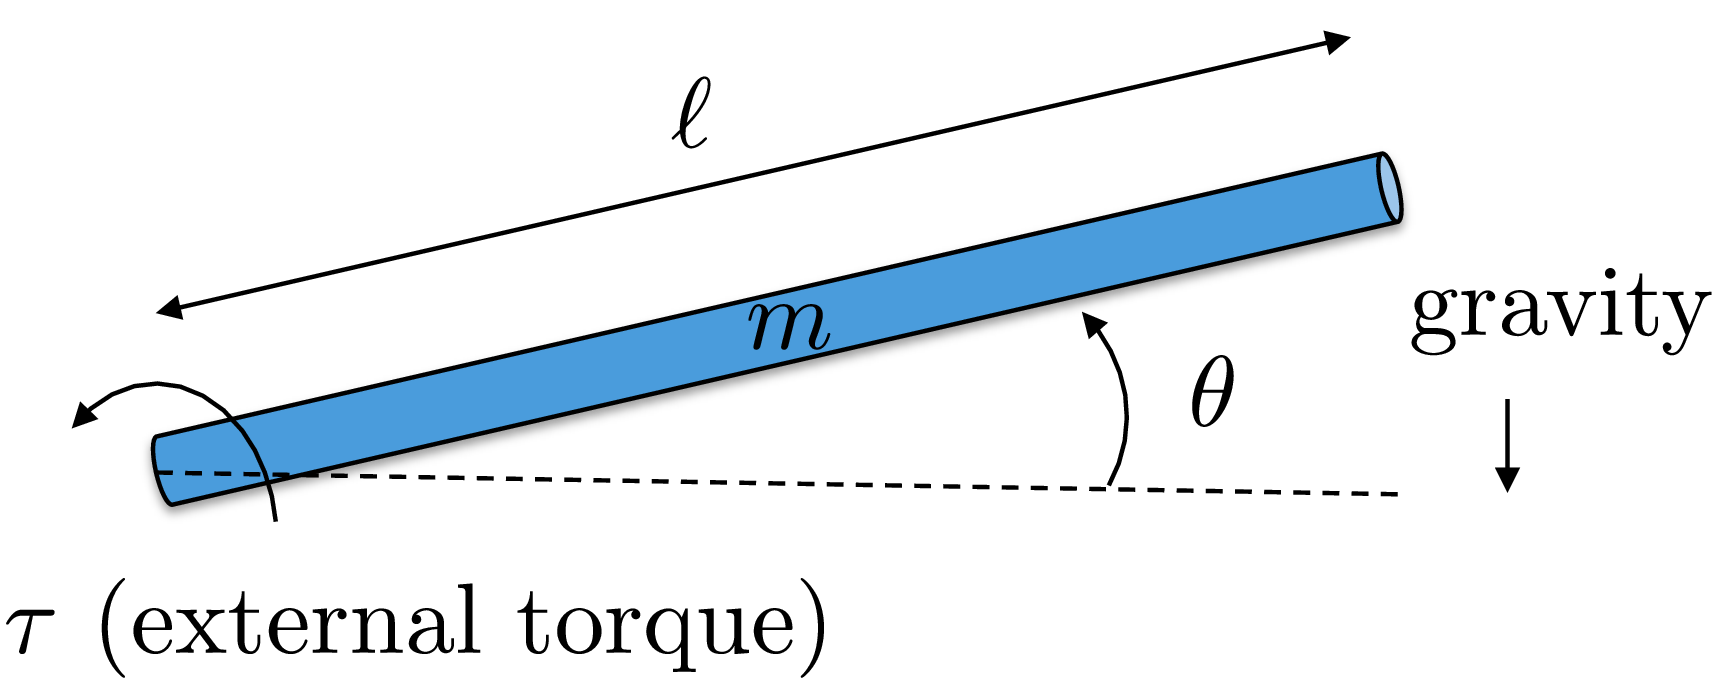
\includegraphics[width=0.6\textwidth]{6_design_studies/figures/hw_arm_defn.pdf}\\
%  \caption{Single Link Robot Arm}
%  \label{fig:int_arm_defn}
%\end{figure}

\begin{wrapfigure}{r}{0.5\textwidth}
  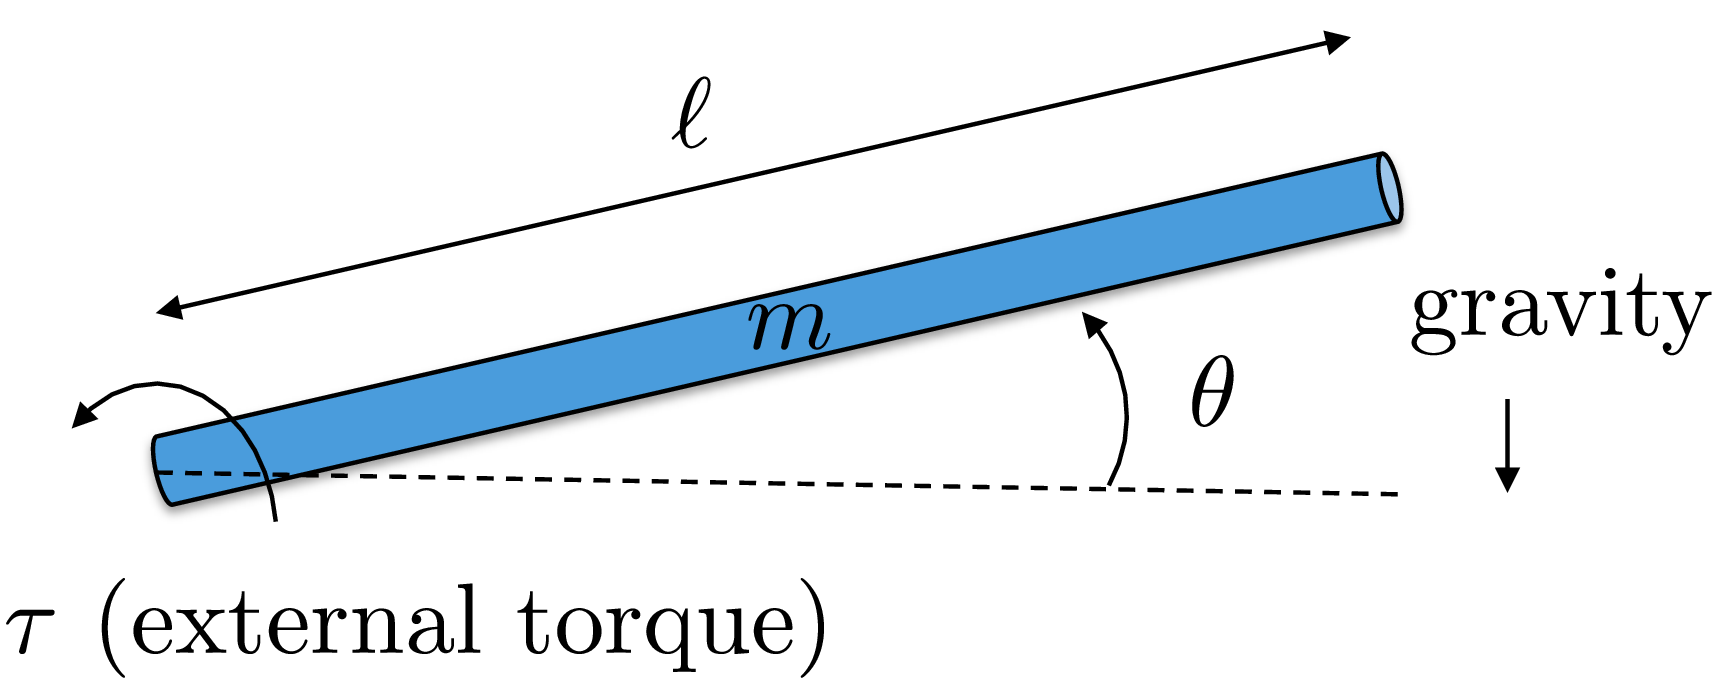
\includegraphics[width=0.49\textwidth]{6_design_studies/figures/hw_arm_defn.pdf}\\
  \caption{Single Link Robot Arm}
  \label{fig:int_arm_defn}
\end{wrapfigure}

Figure~\ref{fig:int_arm_defn} shows a single link robot arm system.  The robot arm has mass $m$ and length $\ell$. The angle of the robot is given by $\theta$ as measured from horizontal to the ground.  The angular speed of the arm is $\dot{\theta}$.  There is an applied torque $\tau$ at the joint.  There is also a damping torque that opposes the rotation of the joint of magnitude, which can be modeled as $-b\dot{\theta}$.

The actual physical parameters of the system are $m=0.5$~kg, $\ell=0.3$~m, $g=9.8$~m/s$^2$, $b=0.01$~Nms.  The torque is limited by $\abs{\tau}\leq 1$~Nm.


